%\newcommand\specialsectioning{\setcounter{secnumdepth}{0}} %定义\specialsectioning命令使\section{}不再编号,用在总结前面使总结、习题和附录不再编号,后面的section不必再使用*
\specialsectioning
\chapter{章节标题}
\label{chap:intro}

\section{引言}
\renewcommand\specialsectioning{\setcounter{secnumdepth}{2}} %定义\specialsectioning命令使\section{}不再编号,用在总结前面使总结、习题和附录不再编号,后面的section不必再使用*
\specialsectioning
\renewcommand\sectionmark[1]{\markright{\thesection  #1}{}}

这是引言


\section{节标题}
\label{xdtz}

这是正文这是正文这是正文这是正文这是正文这是正文这是正文这是正文。\textcolor{myblue}{\textbf{相对突出。}}\snote{这是旁注。这里的相对指的是 XX}这是正文这是正文这是正文。这是正文这是正文这是正文。这是正文这是正文这是正文。

\subsection{小节标题}
\label{computer}



%\textcolor{myblue}{\textbf{1. 用机器解放重复计算的双手 } }
\subsubsection{\textcolor{myblue}{\textbf{1. 小标题 }}}
1231231231231i哦Sharpe文化


\begin{figure}[H]
	\begin{center}
		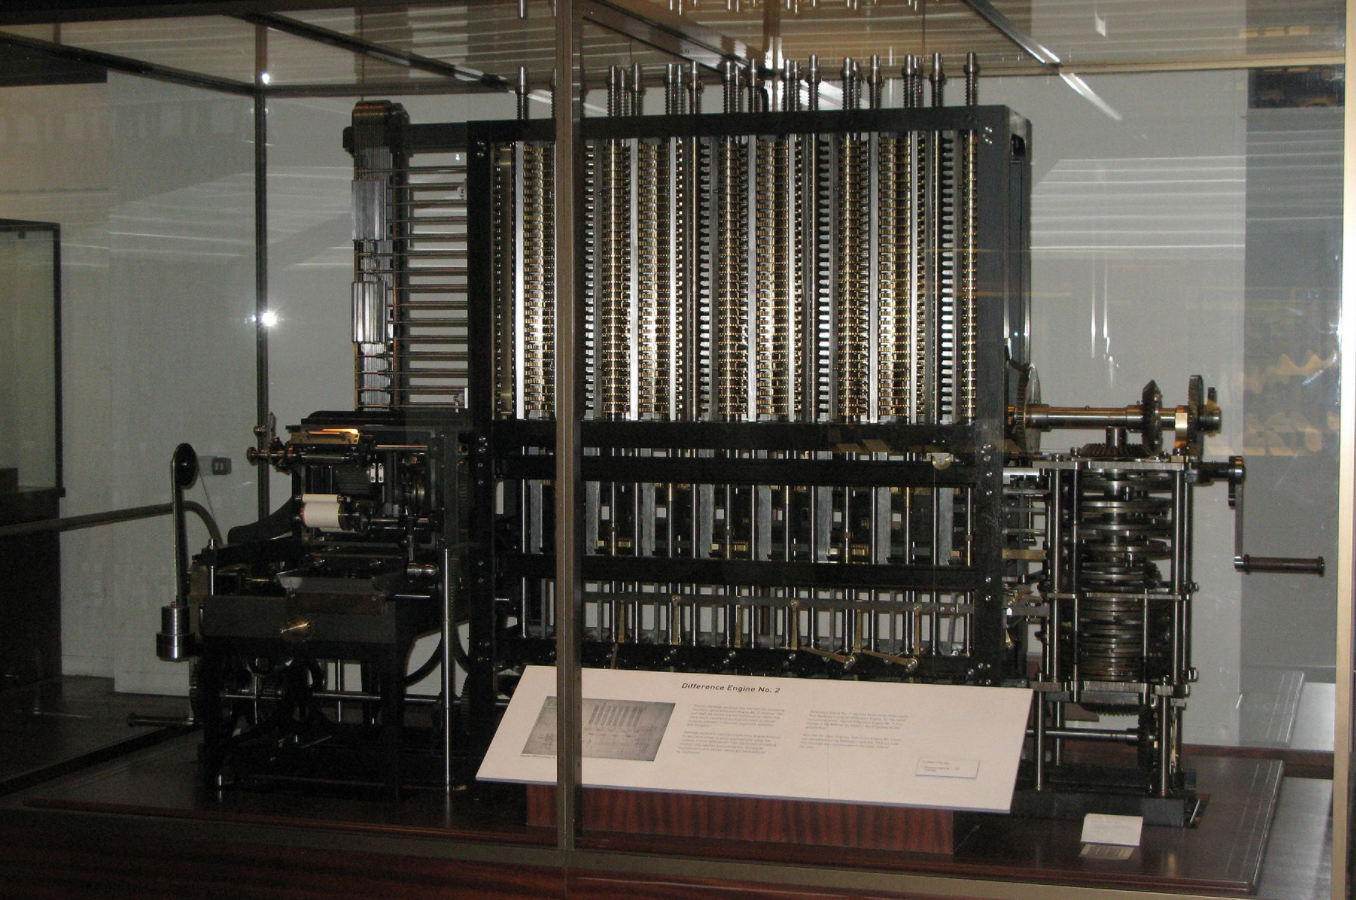
\includegraphics[width=0.6\columnwidth]{Chapter1/graph/差分机2号.png} \\
	\end{center}
	\vspace{-10pt}
	\caption{差分机2号} \label{fig:fenxiji}
	\vspace{-10pt}
\end{figure}




















\section{总结}
\label{xj_ch2}



%\bibliographystyle{unsrt}
%\bibliography{Chapter1/myref}
%\begin{thebibliography}{999}\label{ckwx}
%   \bibitem{ref1}
%	詹姆斯·格雷克. 信息简史[M]. 高博,译. 北京:人民邮电出版社, 2013.
%	\bibitem{ref2}
%	Turing A M. On Computable Numbers, with an Application to the Entscheidungsproblem[J]. Proceedings of the London Mathematical Society, 1937, 2-42(1) : 230–265.
%	\bibitem{ref3}
%	迈克尔·斯韦因, 保罗·弗赖伯格.硅谷之火:个人计算机的诞生与衰落[M]. 陈少芸,成小留,朱少容,译. 3版. 北京:人民邮电出版社, 2019.
%	\bibitem{bianma}
%	查尔斯·佩措尔德. 编码·隐匿在计算机软硬件背后的语言[M]. 左飞,薛佟佟,译. 北京:电子工业出版社, 2012.
%	
%%	https://www.sohu.com/a/154639163_609380,https://www.linkresearcher.com/information/807836f7-989f-4eb5-87e2-f7ceff8e108d(克格勃事件)
%\end{thebibliography}

%\newpage
\section{习题}
%\markboth{习题}{习题}

\begin{enumerate}
	\item {习题1}
	\item {习题2}

\end{enumerate}


